\documentclass{beamer}
\usetheme{CambridgeUS} % replace it with Boadilla if you want no section bar
%\usecolortheme{crane} % other ones: dove, dolphin, rose, seahorse, orchid, crane, seagull, lily, wolverine
%\usefonttheme{serif} 
\usefonttheme[onlymath]{serif} % uncomment if you want it just for math

\setbeamertemplate{navigation symbols}{}  % comment to have nagivation

\usepackage[compress,comma,authoryear]{natbib}
\usepackage{tikz}
\usetikzlibrary{mindmap,trees}
\usepackage{amsmath,mathtools}
\usepackage{amsthm}
\usepackage{booktabs}
\usepackage{graphicx,epstopdf}
\usepackage{hyperref}


\definecolor{blue}{RGB}{0,114,178}
\definecolor{orange}{RGB}{213,94,0}
\definecolor{red}{RGB}{190,0,0}
\definecolor{yellow}{RGB}{240,228,66}
\definecolor{green}{RGB}{0,158,115}
\definecolor{Lblue}{RGB}{0,197,155}
\definecolor{Dblue}{RGB}{0,76,119}
\definecolor{Lgreen}{RGB}{180,255,230}

\hypersetup{
	colorlinks=false,
	linkbordercolor = {white},
	linkcolor = {blue}
}
\definecolor{MyBackground}{RGB}{245,245,245}

\setbeamercolor{frametitle}{fg=blue}
\setbeamercolor{title}{fg=blue}
\setbeamertemplate{footline}[frame number]
\setbeamertemplate{navigation symbols}{} 
\setbeamertemplate{itemize item}[circle]%{$\bigstar$}
\setbeamertemplate{itemize subitem}{$\bigstar$}
\setbeamercolor{itemize item}{fg=blue}
\setbeamercolor{itemize subitem}{fg=blue}
\setbeamercolor{enumerate item}{fg=blue}
\setbeamercolor{enumerate subitem}{fg=blue}
\setbeamercolor{button}{bg=MyBackground,fg=blue}
\setbeamercolor*{palette primary}{use=structure,fg=blue,bg=white}
\setbeamercolor*{palette secondary}{use=structure,fg=white,bg=Dblue}
\setbeamercolor*{palette tertiary}{use=structure,fg=white,bg=blue}
\setbeamercolor*{palette quaternary}{fg=white,bg=black}
\setbeamercolor*{palettes quaternary}{fg=white,bg=Lgreen}
%\setbeamercolor{titlelike}{parent=structure,bg=Lgreen}
%\setbeamercolor{title in head/foot}{bg=Lgreen,fg=orange}

\setbeamertemplate{enumerate item}{%
	\usebeamercolor[bg]{item projected}%
	\raisebox{1.5pt}{\colorbox{blue}{\color{fg}\footnotesize\insertenumlabel}}%
}




\begin{document}
	\title[Econometrics 2]{Econometrics 2 (M.Sc.)}
	\subtitle{Difference-in-difference}
	\author[Mohammad Hoseini]{Mohammad Hoseini}
	
	%\institute[IMPS]{Institute for Management and Planning Studies (IMPS)}
	
	
\date[Spring 2024]{Spring 2024 \\
	\vspace{10pt} @metrics2
}

	
\begin{frame}[plain]
	\titlepage
\end{frame}

\section{Difference-in-Difference}
\subsection{Introduction}

\begin{frame}{Outline}

\begin{enumerate}
	\item Introduction
	\item Diff-in-diff regressions
	\item Parallel trend assumption
	\item Two-way fixed effects
	\item Synthetic control 	
\end{enumerate}\bigskip


\end{frame}

\begin{frame}{Motivation}
In the previous lectures, we learn panel fixed effect models. \medskip

The data requirement of FE model is demanding (panel of same units over time.)\medskip

Many times the regressor of interest varies only at a group level (state, cohort, etc.) which is a more aggregated level:
\begin{itemize}
\item state policies regarding health care benefits
\item minimum wages change across states
\item Tax policies across industries
\end{itemize}
In these circumstances, the source of omitted variables bias is unobserved variables at the group and time level.\medskip

We can use repeated cross-sections to make pseudo-panels of groups in these cases $\rightarrow$ much easier to find data
\end{frame}

\begin{frame}{FE vs. diff-in-diff}

\[y_{it} = a_i+ b_t + \beta D_{it}+u_{it} \]
Assume we have a binary treatment $D=0,1$. In terms of potential outcome model the above fixed effect regression assumes
\[ E[y^0_{it}|i,t]=a_i+b_t \ \text{  and  } \ E[y^1_{it}|i,t]=a_i+b_t+\beta  \]
In diff-in-diff, units are divided to multiple groups $s$ and treatment happens to the groups like state, industry, etc. 
\[ E[y^0_{ist}|s,t]=c_s+b_t \ \text{  and  } \ E[y^1_{ist}|s,t]=c_s+b_t+\beta  \]
While the basic strategy is the same as FE, the data requirements are much less. We don't need a panel of repeated observations on unit $i$.

Repeated cross-sections sampling from the same aggregate units $s$ are sufficient.
\end{frame}

\subsection{Assumptions and estimation}
\begin{frame}{Difference-in-Difference }
Comparing the difference between treatment and control groups before and after a treatment, such as a policy change.\medskip

Two-groups of $i$'s: Treatment ($T$) and Control ($C$) in two-periods 1, 2. \medskip

Treatment group in period 2 is the subject of the treatment.
\pause
\begin{itemize}
\item $C_1$: $C$ attributes
\item $C_2$: $C$ attributes + broad economic changes
\item[$\rightarrow$] $C_2-C_1=$ broad economic changes
\pause
\item $T_1$: $T$ attributes
\item $T_2$: $T$ attributes + broad economic changes + treatment effect
\item[$\rightarrow$] $T_2-T_1=$ broad economic changes + treatment effect
\pause
\item[$\rightarrow$] Diff-in-diff: \textbf{$(T_2-T_1)-(C_2-C_1)=$ treatment effect.} 
\end{itemize}
\end{frame}


\begin{frame}{Difference-in-Difference estimation}
Estimation:  \[y_{ist}=\alpha+\gamma_s+\lambda_t+\beta D_{st}+\varepsilon_{ist}\quad\rightarrow \beta=\text{treatment effect} \]
$\gamma$ group dummy: =0 if control and =1 if treatment group.

$\lambda$ time dummy: =0 if first and =1 if second period.

$D$ treatment dummy: =1 for treatment group after treatment =0 othw.
\[C_1=\alpha,\quad C_2=\alpha+\lambda,\quad T_1=\alpha+\gamma,\quad T_2=\alpha+\lambda+\gamma+\beta\]
$\Rightarrow \ (T_2-T_1)-(C_2-C_1)=\beta$\medskip

We can generalize this when there are $S>2$ groups and $T>2$ periods and treatment happens for each group in different time.

Then $D_{st}$ =1 for $s$'s that are under treatment at time $t$ and 0 otherwise.  

\end{frame}

\begin{frame}{Parallel trends in diff-in-diff}
The heart of DD setup is an additive structure or \textit{parallel trends} for potential outcomes in the no-treatment state.

ID assumption: $E[y^0_{ist}|s,t]=\gamma_s+\lambda_t$ ,    $E[y^1_{ist}-y^0_{ist}|s,t]=\beta$

%The identification assumption in diff-in-diff: in the absence of treatment, the outcome is equal to the sum of a time-invariant group effect (S1 or S2) and a time effect which is invariant across groups (T1 or T2).
\begin{center}
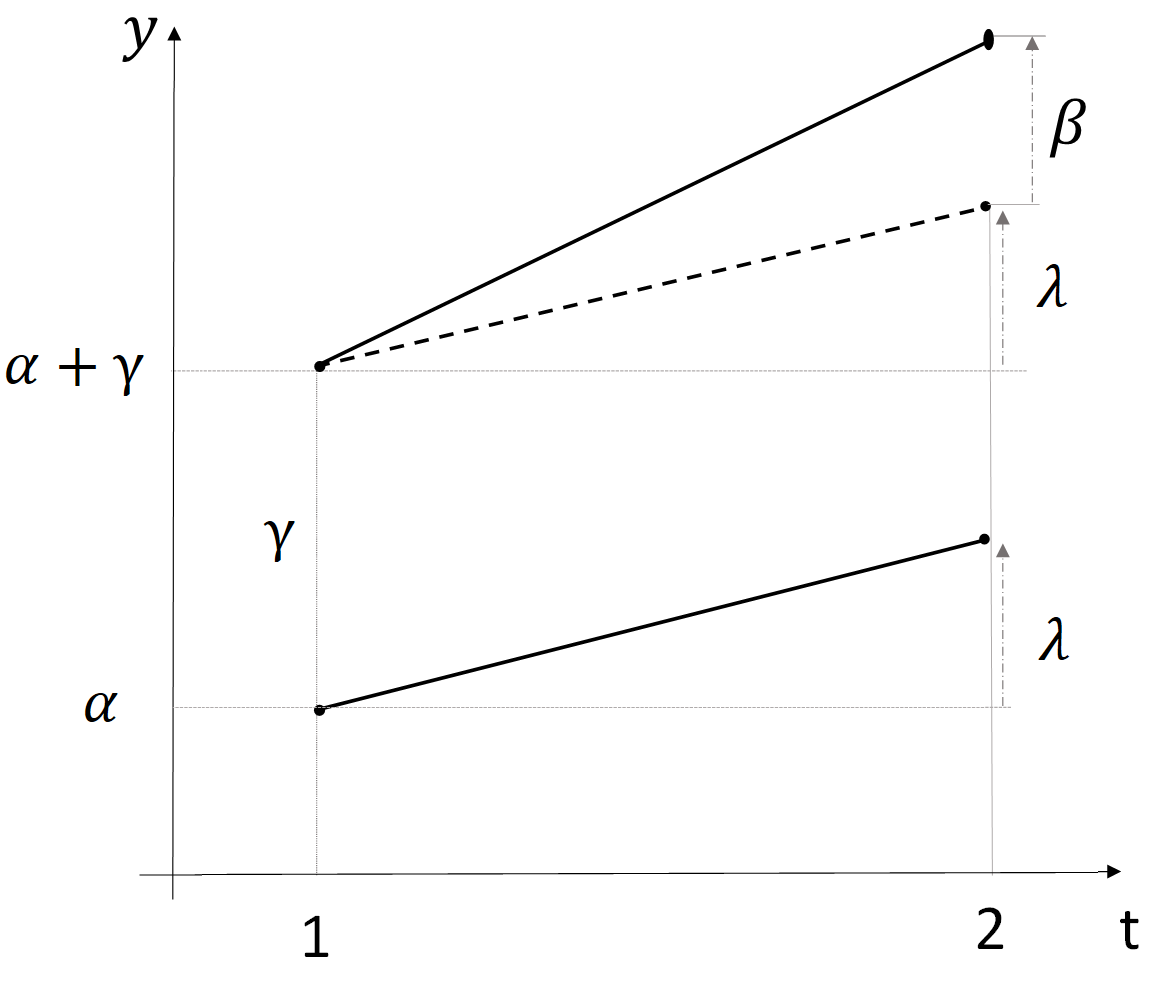
\includegraphics[width=0.6\textwidth]{./Figures/trend.png}
\end{center}

\end{frame}

\begin{frame}{Parallel trend assumption}
	
The key assumption for any DD strategy is that the outcome in treatment and control groups would follow the same time trend in the absence of the treatment.\bigskip

This does not mean that they have to have the same mean of the
outcome!\bigskip

Common trend assumption is difficult to verify but one often uses pre-treatment data to show that the trends are the same.\bigskip

Even if pre-trends are the same one still has to worry about other policies changing at the same time.\bigskip

Another important assumption in DiD is exogeneity of treatment otherwise reverse causality problem. 
\end{frame}


\begin{frame}{Parallel trends with more periods and groups}
The ID assumption: counterfactual trend (the dashed line) is parallel to the control group trend and the effect of treatment is permanent. 

%Common trend assumption is diffcult to verify but one often uses pre-treatment data to show that the trends are the same.
%Even if pre-trends are the same one still has to worry about other policies changing at the same time.
\begin{center}
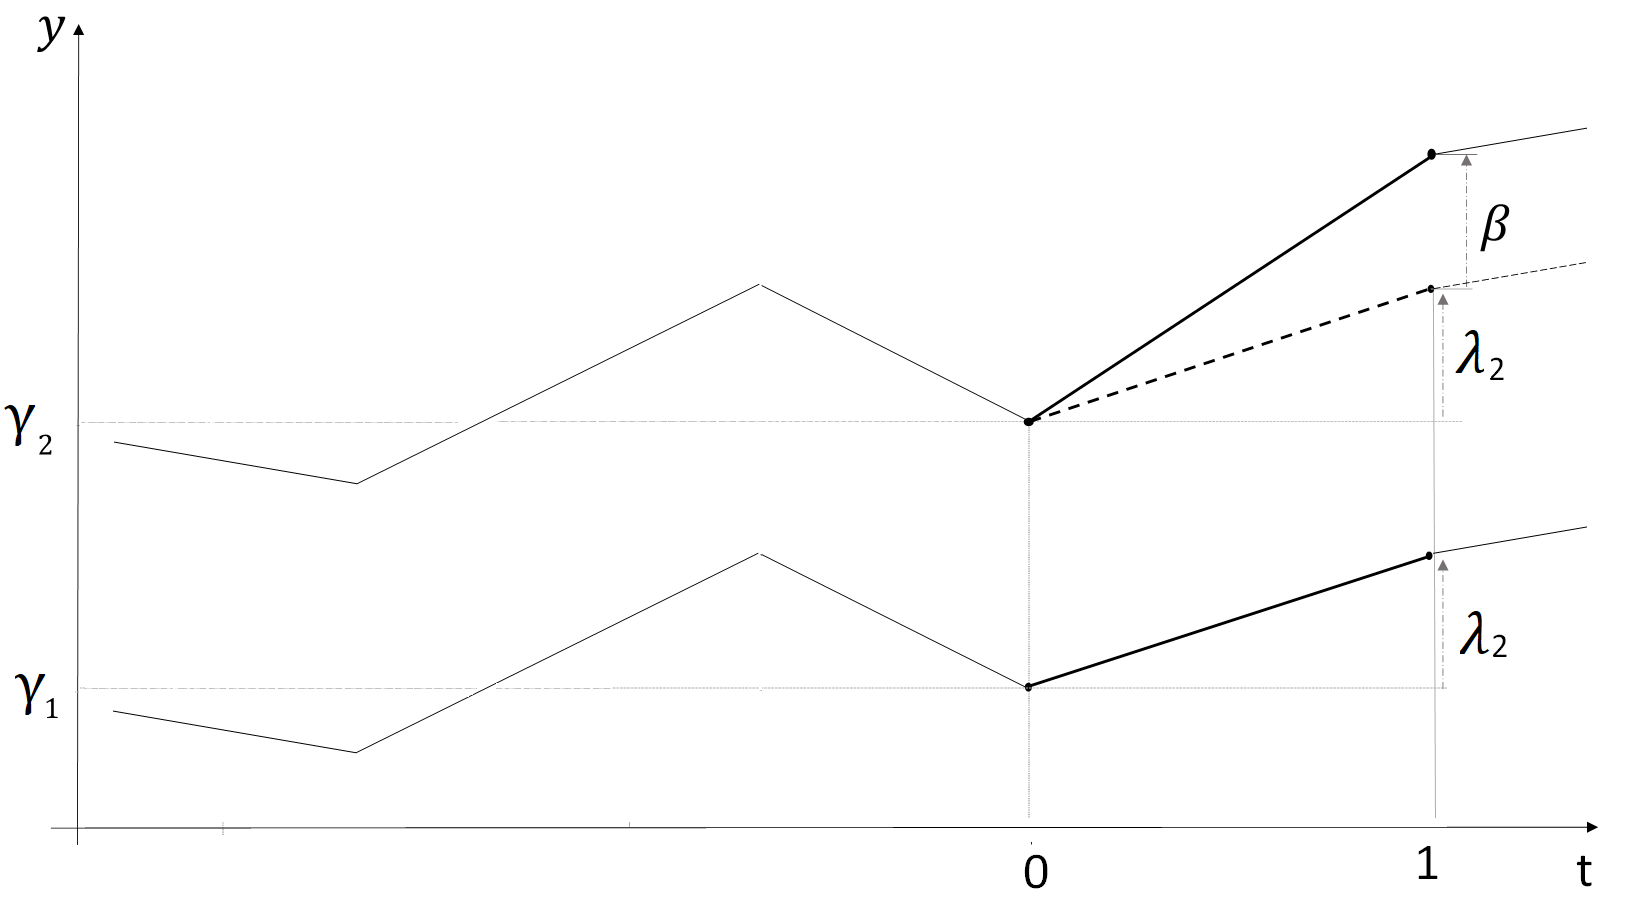
\includegraphics[width=0.9\textwidth]{./Figures/trends.png}
\end{center}
\end{frame}

\begin{frame}{Standard Errors in Diff-in-diff}
It is common to diff-in-diff for many periods and not only before and after the treatment.\medskip

The treatment variables is normally changes only at group level (say state) and like other panel data outcome variables are often serially correlated.\medskip

Bertrand, Duflo, and Mullainathan (2004) point out that conventional standard errors often severely understate the standard deviation of the diff-in-diff estimators and provide some solution:
\begin{itemize}
\item Cluster standard errors at group level.
\item Aggregate data at pre- and post-treatment periods.
\item Bootstrap standard errors.
\end{itemize}
\end{frame}

\subsection{Examples}
\begin{frame}{\cite{card1994minimum}}
The effect of minimum wage on employment: 
In a competitive labor market, higher minimum wage reduces labor demand and equilibrium employment.\medskip

In February 1992 New Jersey increased the state minimum wage from \$4.25 to \$5.05. Pennsylvania's minimum wage stayed at \$4.25.\medskip

They surveyed about 400 fast food stores both in NJ and in PA both before and after the minimum wage increase in NJ.
\begin{figure}
\centering

\includegraphics[width=0.4\linewidth]{./Figures/card-krueger}
\label{fig:card-krueger}
\end{figure}

\end{frame}

\begin{frame}{\cite{card1994minimum}}
Diff-in-diff identification assumptions:
\begin{itemize}
\item $Y^0_{ist}:$  employment in restaurant $i$, state $s$, time $t$ if low min-wage.
\item $Y^1_{ist}:$ employment in restaurant $i$, state $s$, time $t$ if high min-wage.
\end{itemize}
\[E[Y^0_{ist}|s,t]=\gamma_s+\lambda_t \ \text{ and }\ E[Y^1_{ist}|s,t]=\gamma_s+\lambda_t+\beta \]
In the absence of a minimum wage change, employment is determined
by the sum of a time-invariant state effect $\gamma_s$ and a year effect $\lambda_t$ that is common across states.
\[Y_{ist}=\gamma_s+\lambda_t+\beta D_{st}+\varepsilon_{ist} \]
$D_{st}$ is a dummy for high-minimum wage states and periods.
\end{frame}

\begin{frame}{\cite{card1994minimum}}
Average employment per store before and after the New Jersey minimum wage increase: min-wage $\uparrow \ \Rightarrow$ employment $\uparrow$?
\footnotesize
\begin{table}
\centering
\begin{tabular}{lccc}
\hline\hline
&PA &NJ &Difference, NJ-PA\\
Variable& (i) &(ii) &(iii)\\
\hline
1. FTE employment before& 23.33& 20.44& -2.89\\
& (1.35)&(0.51)& (1.44)\\
2. FTE employment after,& 21.17& 21.03& -0.14\\
& (0.94) &(0.52) &(1.07)\\
3. Change in mean FTE employment &-2.16& 0.59& \textbf{2.76}\\
&(1.25) &(0.54)& \textbf{(1.36)}\\
\hline\hline
\end{tabular}
\end{table}

Adapted from \cite{card1994minimum}, Table 3. The
table reports average full-time equivalent (FTE) employment at
restaurants in Pennsylvania and New Jersey before and after a
minimum wage increase in New Jersey. The sample consists of
all stores with data on employment. Employment at six closed
stores is set to zero. Employment at four temporarily closed stores
is treated as missing. Standard errors are reported in parentheses.
\end{frame}

\begin{frame}{\cite{card2000minimum}}
How convincing is this evidence against the standard labor-demand story? Is the common trend assumption ok?\medskip

Using administrative data \cite{card2000minimum} show that it is not.
\begin{figure}
\centering
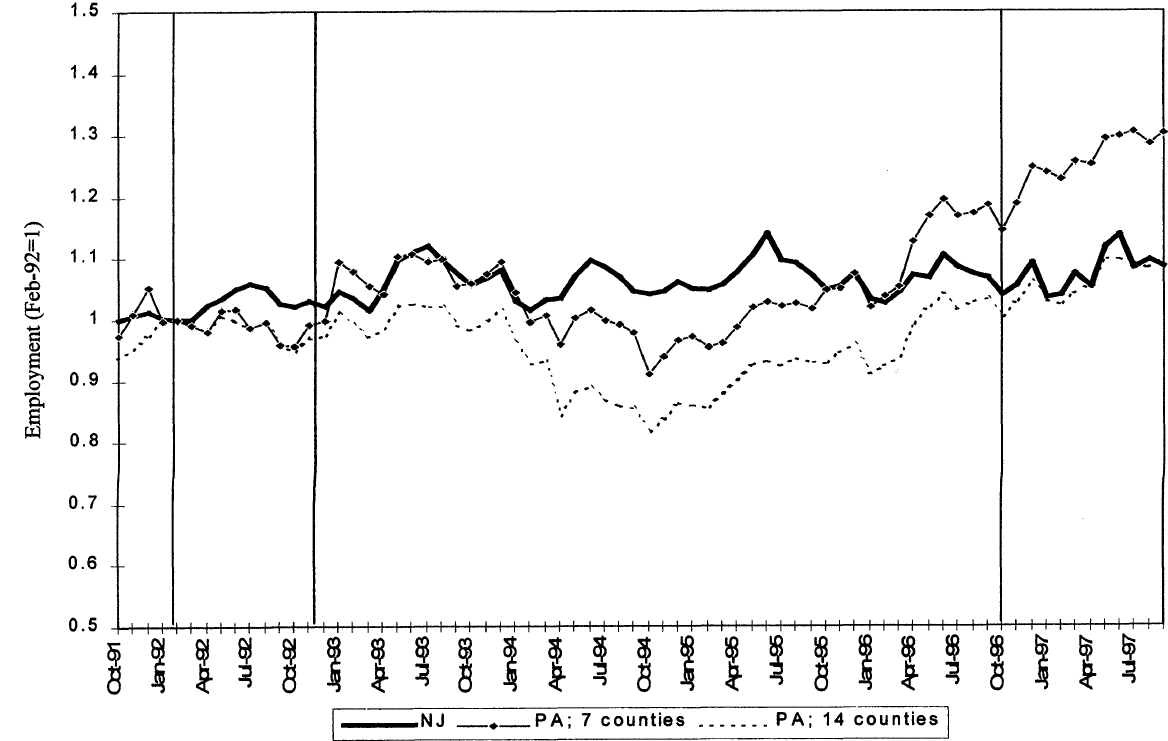
\includegraphics[width=0.75\linewidth]{./Figures/card-krueger2}
\end{figure}

\end{frame}


\begin{frame}{\cite{jayaratne1996finance}}
	An example of multiple periods and treatment and multiple time.\medskip
	
	How banks can affect growth?\medskip
	
	Treatment: Banking deregulation across the U.S. states between 1970-95 with different timings.
	\begin{center}
		$g_{it}=\mu_i+\eta_t+\beta D_{it}+\varepsilon_{it}$
	\end{center}
	
	\begin{itemize}
		\item $g_{it}=y_{it}/y_{it-1}$ growth, $D_{it}$ is one if state $i$ is deregulated at time $t$.
		\item At any point of time, T: deregulated states, C: not deregulated yet.
		\item $\beta>0$ is significant, so bank deregulation fostered growth 
	\end{itemize}
	Deregulations were independent across states? biased $\beta$?\medskip
	
	Remember: Cluster standard errors when there are multiple times.
\end{frame}


\begin{frame}{Two-way fixed effect}
\cite{card1994minimum} was an example of 2x2 difference-in-difference: there are two groups, and treatment occurs at a single point in time.\bigskip 
	
\cite{jayaratne1996finance} is an example of treatments staggered treatment or a ``rollout'' design: treatments are implemented at different times.\bigskip 
	
	The regression of \cite{jayaratne1996finance} is also called ``two-way'' fixed effects: using fixed effects for group and time periods.\bigskip 
	
%	Recent works show that this approach with DiD can heavily bias results if treatment effects differ across groups. See Goodman-Bacon (2019) and Callaway and Sant'anna (2019).
\end{frame}

\begin{frame}{\cite{autor2003outsourcing}}
	includes both leads and lags in a DD model analyzing the effect of increased employment protection on the firm's use of
	temporary help workers.\medskip
	
	In the US employers can usually hire and fire workers at will.\medskip
	
	Some states courts have made some exceptions to this employment at will rule and have thus increased employment protection.\medskip
	
	Different states have passed these exceptions at different points in time.\medskip
	
	The standard thing to do is to normalize the adoption year to 0.\medskip
	
	Autor then analyzes the effect of these exceptions on the use of temporary help workers.
\end{frame}

\begin{frame}{\cite{autor2003outsourcing}}
	$y_{it}=\mu_i+\eta_t+\delta_{-2} D_{i,-2}+\dots+\delta_{0} D_{i,0}+\delta_{+1} D_{i,+1}+\dots+\delta_{\ge4} D_{i,\ge4}+\varepsilon_{it}$
	\begin{figure}
		\centering
		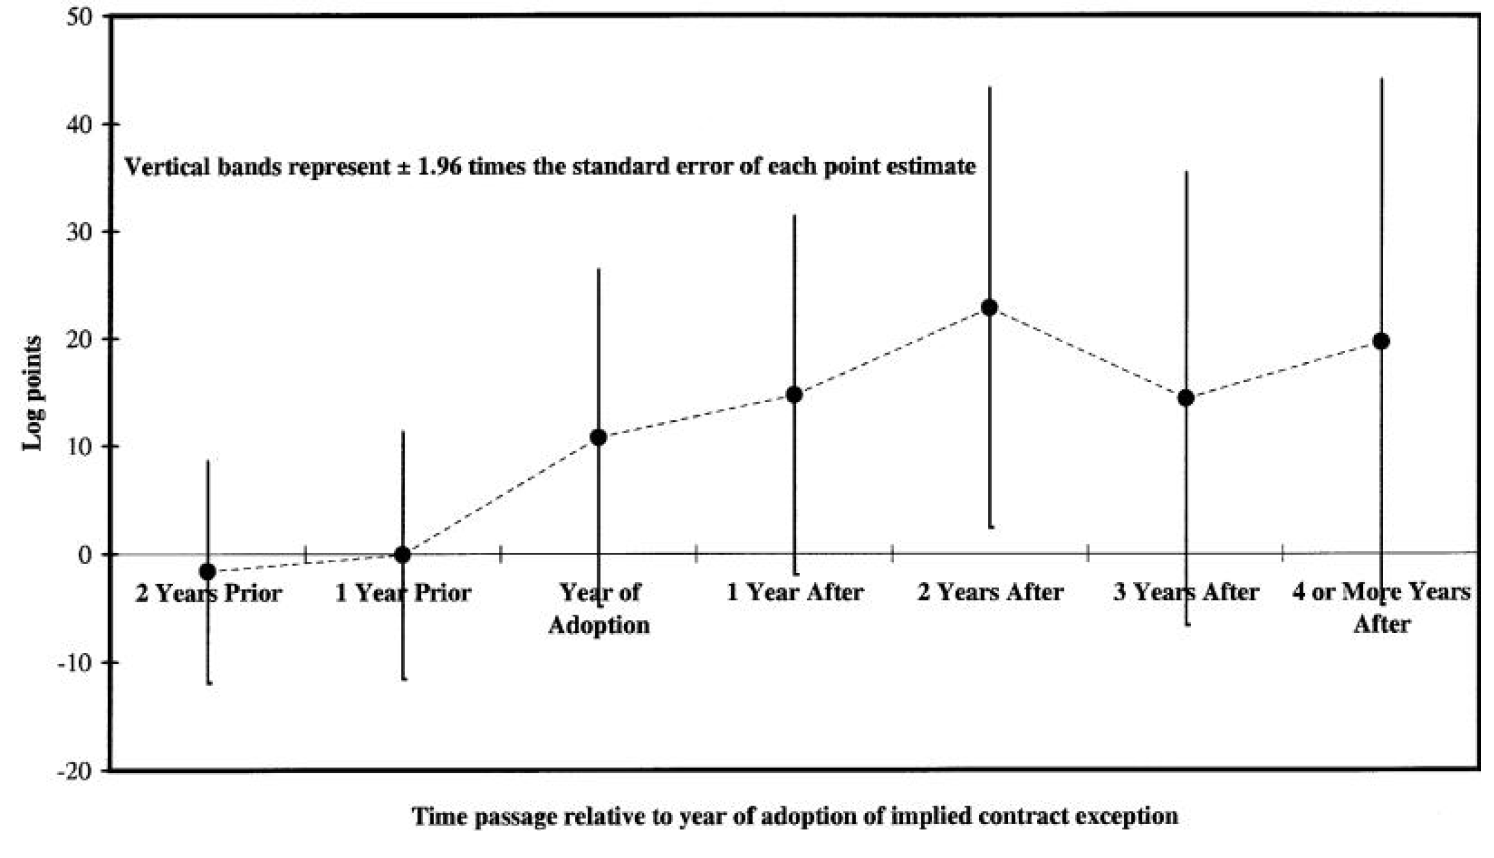
\includegraphics[width=0.7\linewidth]{./Figures/autor2003}
	\end{figure}
	Parallel trends assumption: The leads are very close to 0 thus no evidence for anticipatory effects.\medskip
	
	The lags show that the effect increases during the first years of the treatment and then remains relatively constant.	
\end{frame}


\begin{frame}{DiD Event Study / Dynamic DiD}
	The last slide's graph is an example of DiD event study, or a Dynamic DID model.\bigskip
	
	When the treatment is staggered -- where the treatment group are treated at different time periods -- you can use this tool in evaluating treatment effects of the pre- and post- treatment periods.\bigskip 
	
	%However, Sun and Abraham (2020) showed that basic DiD event-study estimation can be biased and propose an alternative estimator. 
\end{frame}

\begin{frame}{Post 2020 DiD literature}
	Recent literature on DiD can be broadly classified as relaxing some components of the canonical DiD setup, with a focus on 
	\begin{itemize}
		\item Multiple periods and staggered treatment timing 
		\begin{itemize}
			\item \cite{de2020two,goodman2021difference,sun2021estimating}, etc. 
			\item a survey paper: \cite{de2023two}
		\end{itemize}
		\item Violations of parallel trends
		\begin{itemize}
			\item \cite{rambachan2023more,callaway2021difference,roth2023parallel}
		\end{itemize}
		%\item Alternative frameworks for inference.
	\end{itemize}
	 
\end{frame}

\begin{frame}{\cite{goodman2021difference} - staggered treatment}
	Consider a treatment with early, late, and never adopters groups.
\begin{center}
	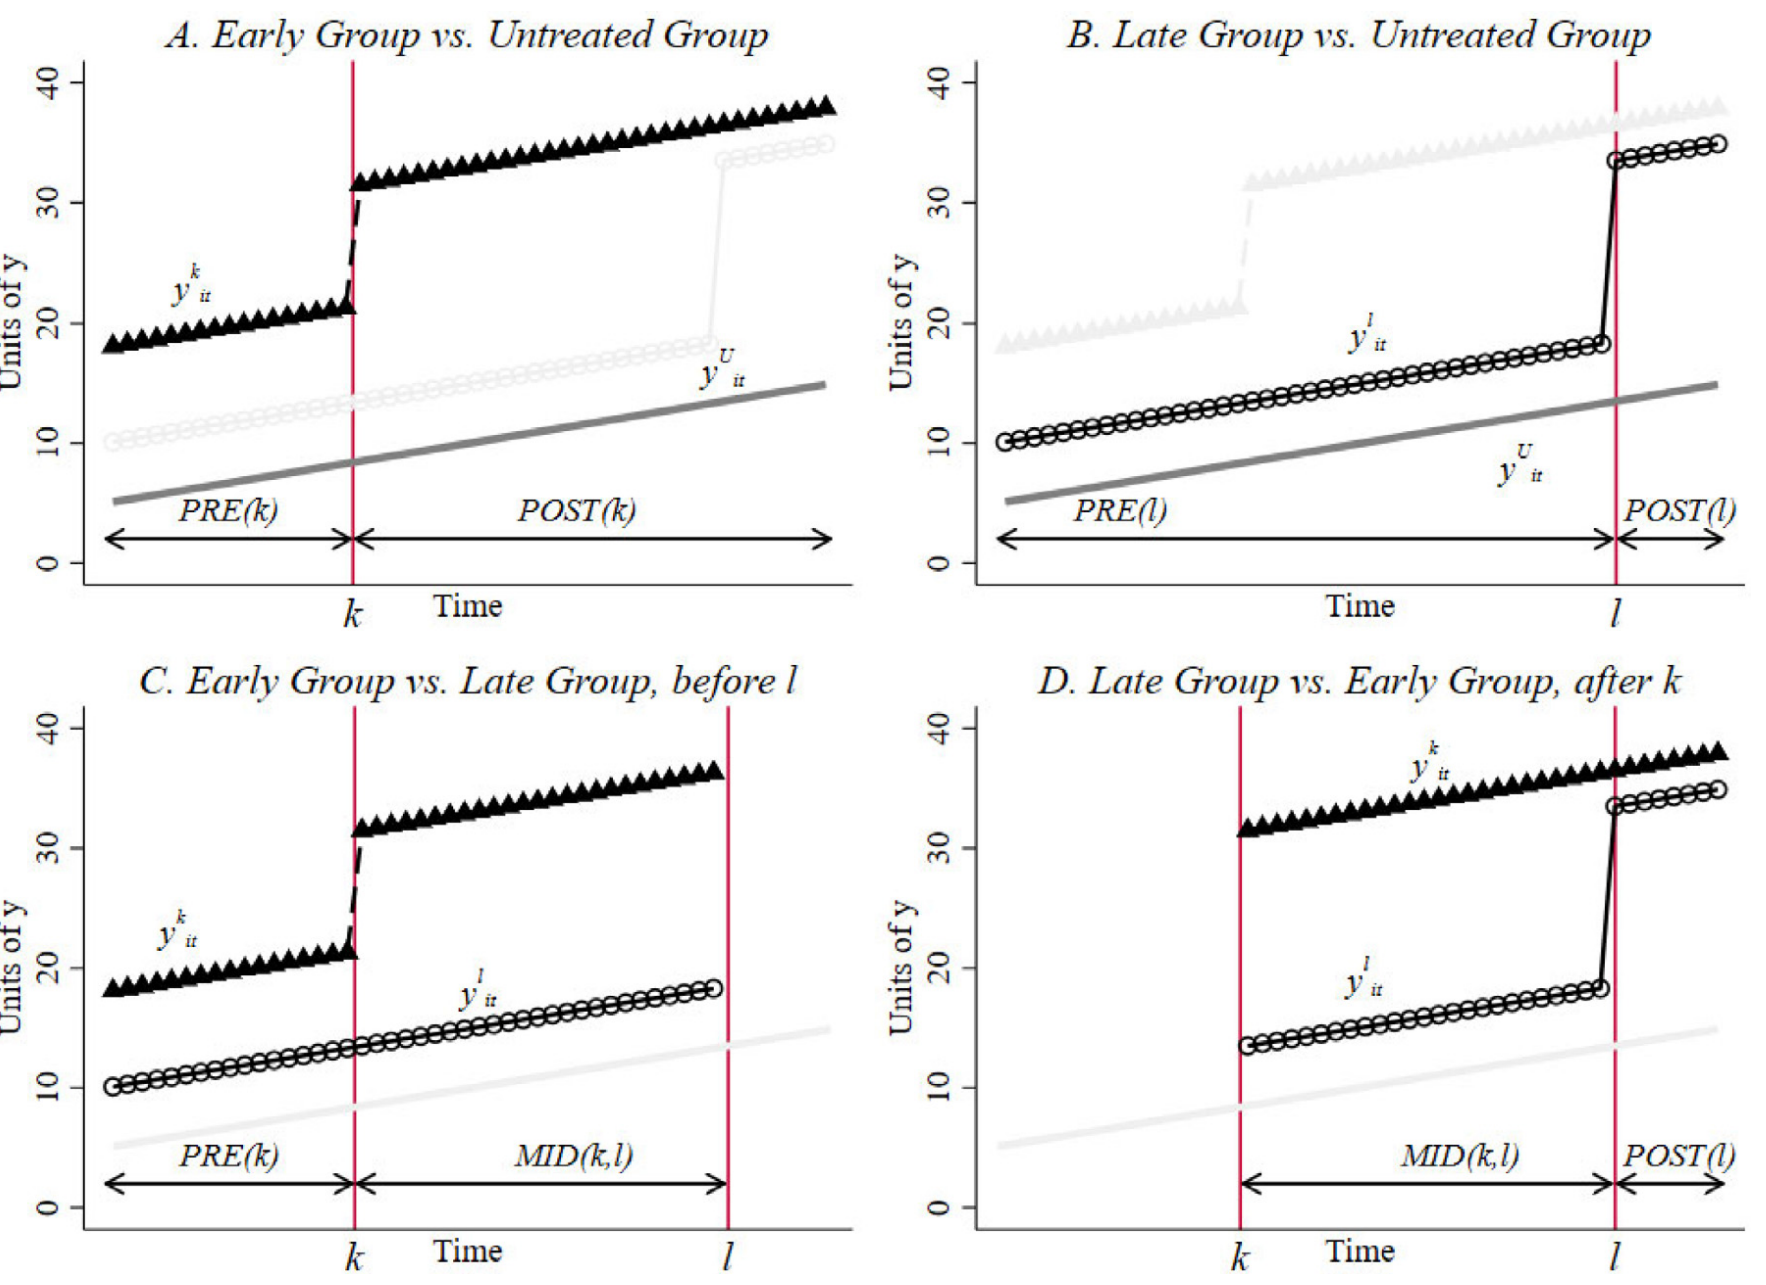
\includegraphics[width=0.8\linewidth]{./Figures/GoodmanBacon2021}
\end{center}
	%In the early time-frame, the late adopters  are ``never treated'', in another the early adopters are ``always treated''.
\end{frame}

\begin{frame}{\cite{goodman2021difference}}
Any two-way fixed effects estimate of DD with variation in treatment timing is a weighted average of 
\begin{enumerate}
	\item comparisons between (relatively) early adopters and later adopters over the periods when the later adopters are not yet treated,
	\item comparisons between early adopters and later adopters over the periods when the early adopters are treated – so that they can be used as a comparison group for the later adopters,
	\item comparisons between different timing groups (e.g., early adopters or later adopters) and the never-treated group, if there is one. 
\end{enumerate}
When treatment effects are heterogeneous across units, in OLS estimation, units that are treated near the middle of the evaluation window receive relatively more weight.\medskip 

When treatment effects change over time within unit, two-way fixed effects estimators are not appropriate, and alternative approaches should be used. 
\end{frame}

\begin{frame}{Limitations of pre-trend tests of parallel trends}
	Parallel pre-trends doesn't necessarily imply parallel (counterfactual) post-treatment
	trends\bigskip
	%If other policies change at the same time as the one of interest — e.g. min wage and UI reform together — can produce parallel pre-trends but non-parallel post-trends
	%Likewise, could be that treated/control groups are differentially exposed to recessions, but there is only a recession in the post-treatment period
	
	Low power: even if pre-trends are non-zero, we may fail to detect it statistically\bigskip
	
	Pre-testing issues: if we only analyze cases without statistically significant pre-trends,	this introduces a form of selection bias %(which can make things worse)
	\bigskip
	
	\cite{rambachan2023more} provides sensitivity analysis: counterfactual post-treatment trends cannot be ``too different'' from the pre-trends\bigskip
	
	\cite{callaway2021difference} suggest a pre-testing approach that extends to settings with staggered adoption
	
	
	
\end{frame}


\begin{frame}{Checklist \citep{roth2023s}}
	\begin{figure}
		\centering
		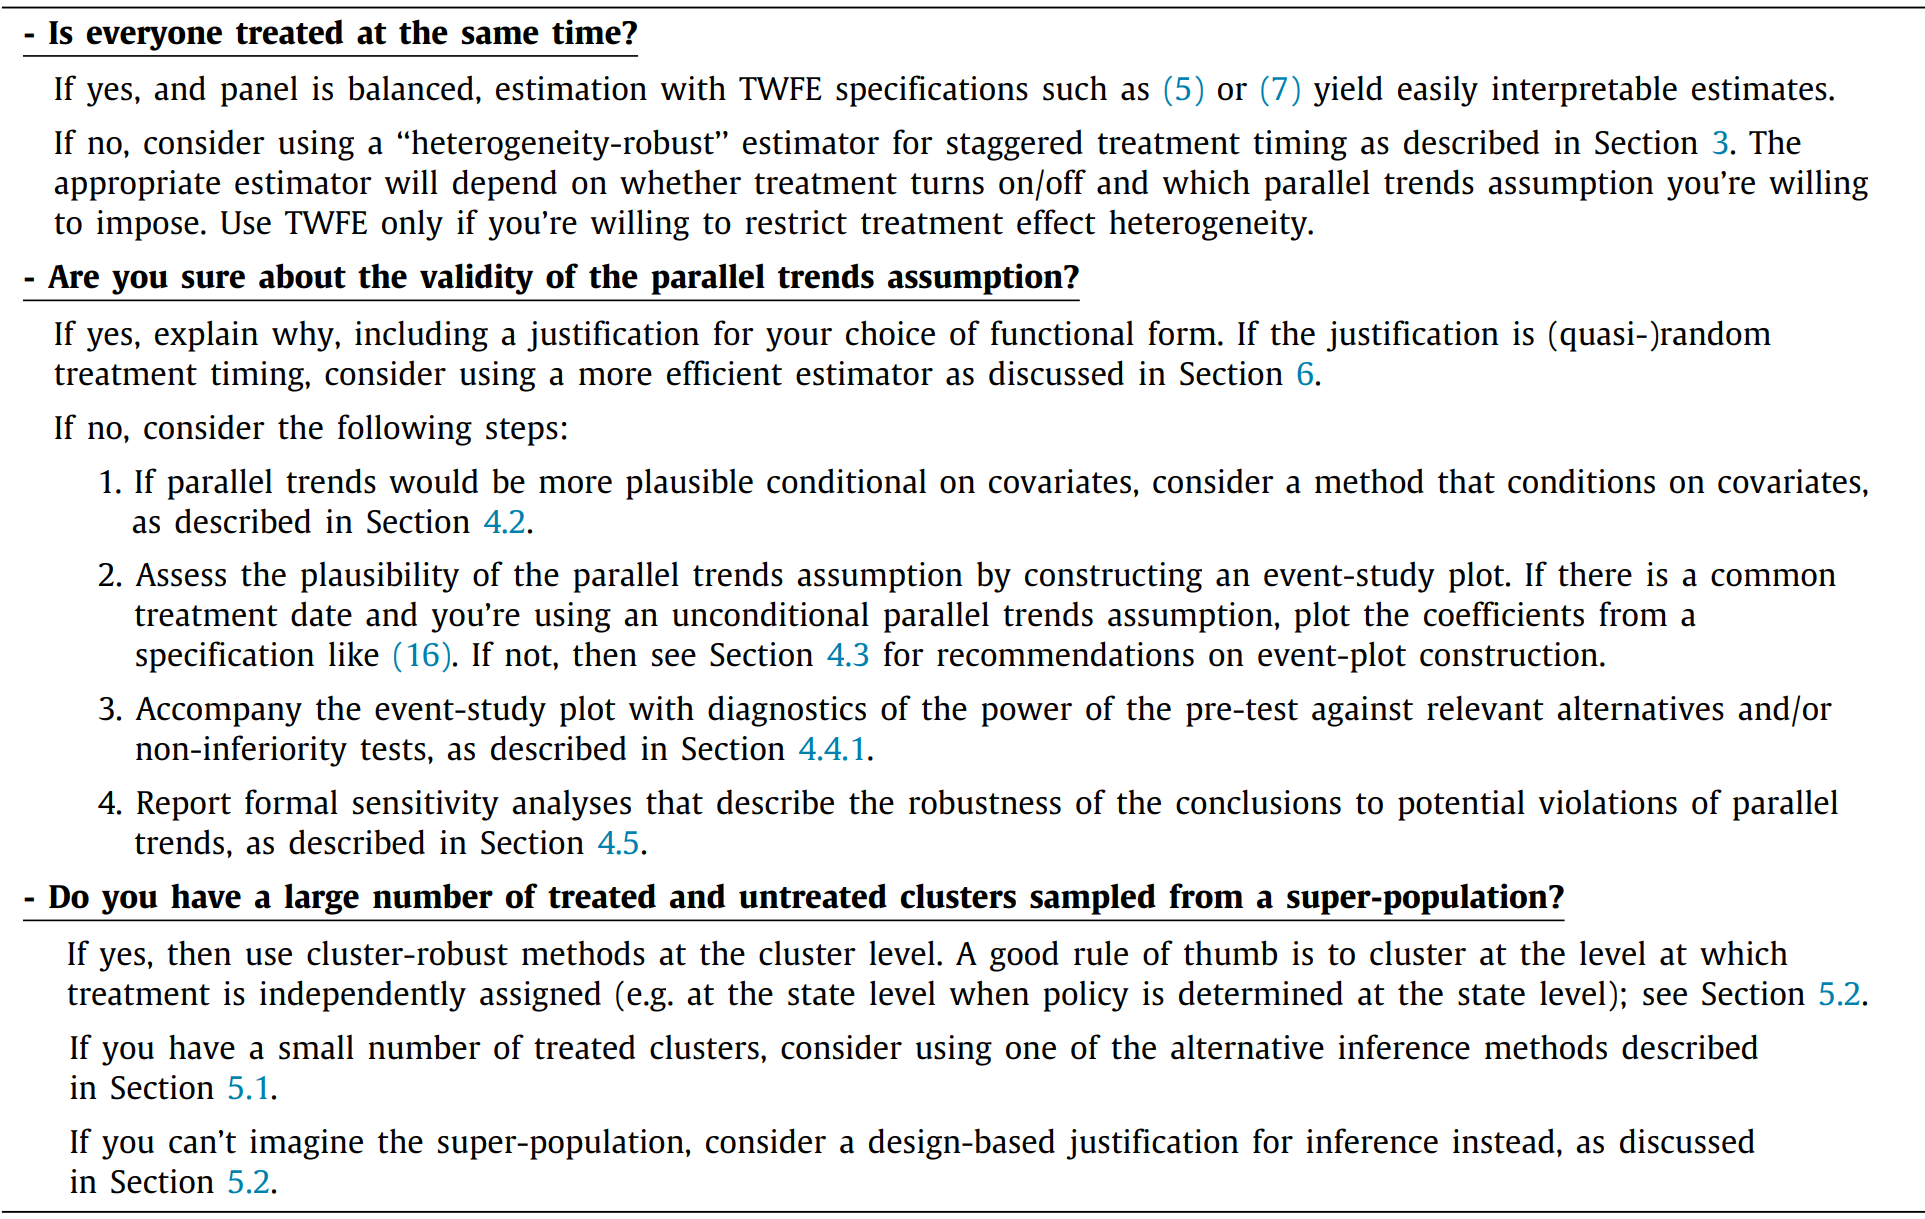
\includegraphics[width=\linewidth]{./Figures/DiDalghorithm.png}
	\end{figure}
\end{frame}

\begin{frame}{Statistical Packages \citep{roth2023s}}
	\begin{figure}
		\centering
		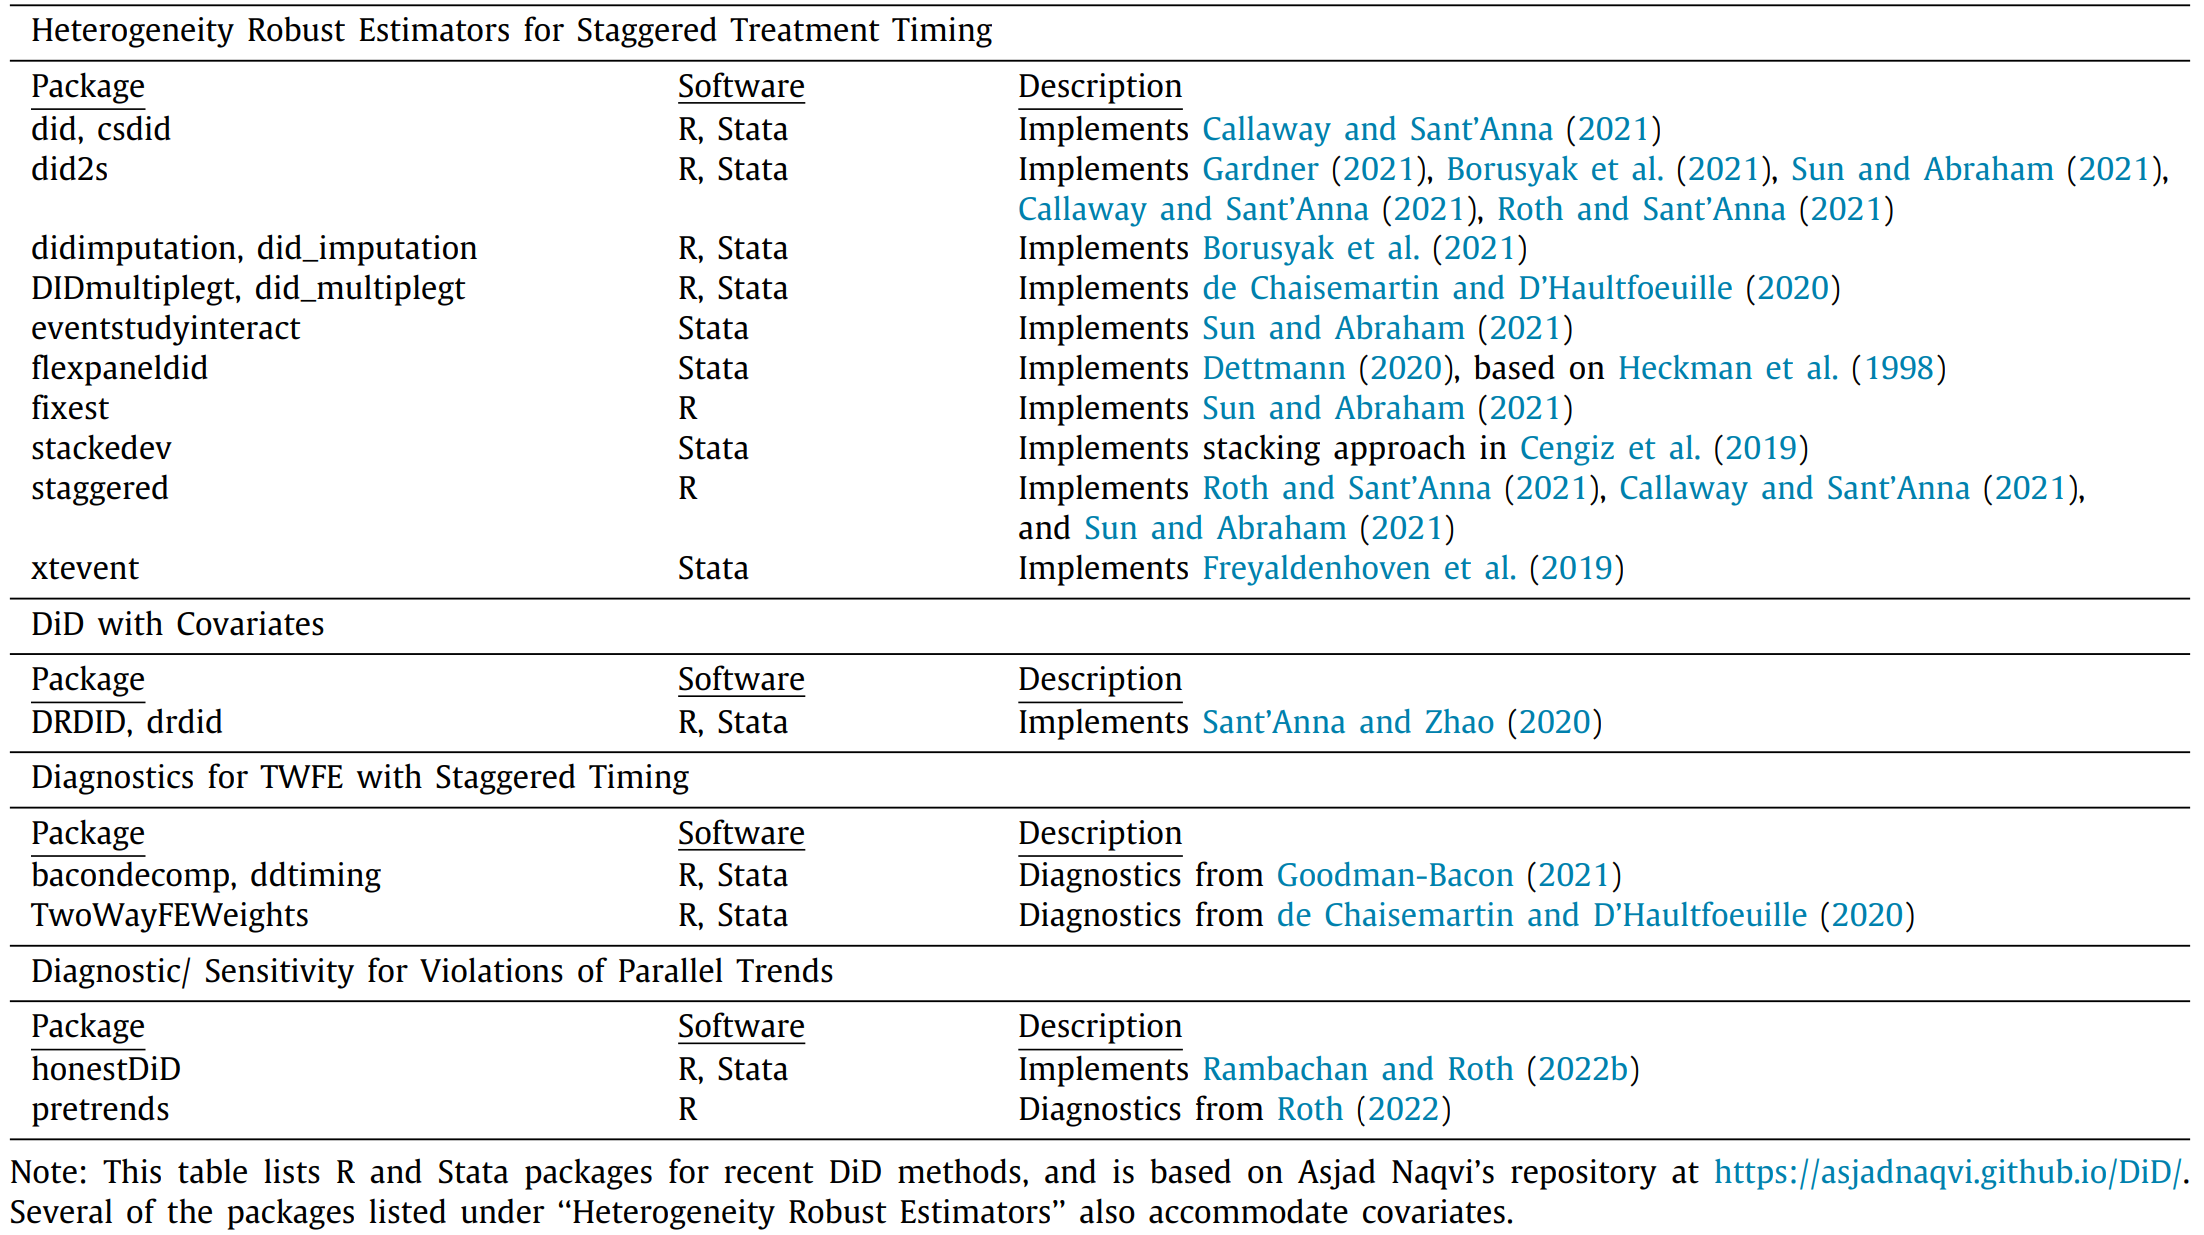
\includegraphics[width=\linewidth]{./Figures/DiDpackages.png}
	\end{figure}
\end{frame}

\subsection{Synthetic Control Group}
\begin{frame}{Synthetic Control Methods}
In some cases, treatment and control groups do not follow parallel trends and standard DiD method would lead to biased estimates.\bigskip

The basic idea behind synthetic controls is that a combination of
units often provides a better comparison for the unit exposed to the intervention than any single unit alone.\bigskip

\cite{card1990impact} used this approach in investigating the effect of Cuban immigration on employment of natives in Florida.\medskip

\cite{abadie2003economic} used a synthetic control method when estimating the effects of the terrorist conflict in the Basque Country using other Spanish regions as a comparison group.

\end{frame}

\begin{frame}{\cite{card1990impact}}
The effect of an influx of immigrants on natives' unemployment\medskip

On April 20th, 1980 the Cuban government allowed Cubans to emigrate to the US, which led to roughly 125,000 Cubans entering the United States through Florida. 
Half of the immigrants settled permanently in Miami, raising the labor force there by seven percent.
\[ \beta=(UN_{Miami 1981}-UN_{Miami 1979})-(UN_{Control 1981}-UN_{Control 1979}) \]  
\cite{card1990impact} uses Atlanta, Los Angeles, Houston and Tampa-st. Petersburg with similar white, black, and non-Cuban Hispanic wages and employment as Miami.\medskip

The event did not negatively impact wages or employment levels of native workers.\medskip

Employment of black males in Miami fell compared to employment of black males in the control
cities, and these differences only rose after the Mariel boatlift.\medskip


\end{frame}

\begin{frame}{\cite{abadie2003economic}}
Whether Terrorism in the Basque Country had a negative effect on its growth.\medskip

They cannot use a standard DiD method because none of the other Spanish regions followed the same time trend as the Basque Country.\medskip

They therefore take a weighted average of other Spanish regions as a
synthetic control group:
\begin{itemize}
\item There are 16 other Spanish regions.
\item $w_1,\dots,w_{16}$ is assigned to each region as weight $\sum_{i=1}^{16}w_i=1$.
\item The optimal weights are found so that they most closely resembles the Basque Country before terrorism.
\item The optimal weights: Catalonia: 0.85, Madrid: 0.15, others: 0.
\end{itemize}
\end{frame}

\begin{frame}{Matching meet DiD}
	The synthetic control method adds matching into DiD.\bigskip
	
	To find weights $w_i$, the distance between treatment and controls are minimized in the pre-treatment period:
	
	\[\min_W || X_{\text{treatment}}-X_{\text{control}}.W|| \]
	
	\begin{itemize}
		\item $X_{\text{treatment}}: n\times 1$, desired covariates 
		\item $X_{\text{control}}: n \times k$, desired covariates for $k$ control groups 
		\item $W: k \times 1$, weight of control groups
	\end{itemize}
	An important feature here is that $X$ can include both lagged outcomes and observable characteristics.
\end{frame}



\begin{frame}{\cite{abadie2003economic}}
The Synthetic Basque Country Looks Similar to the actual one.
\begin{figure}
\centering
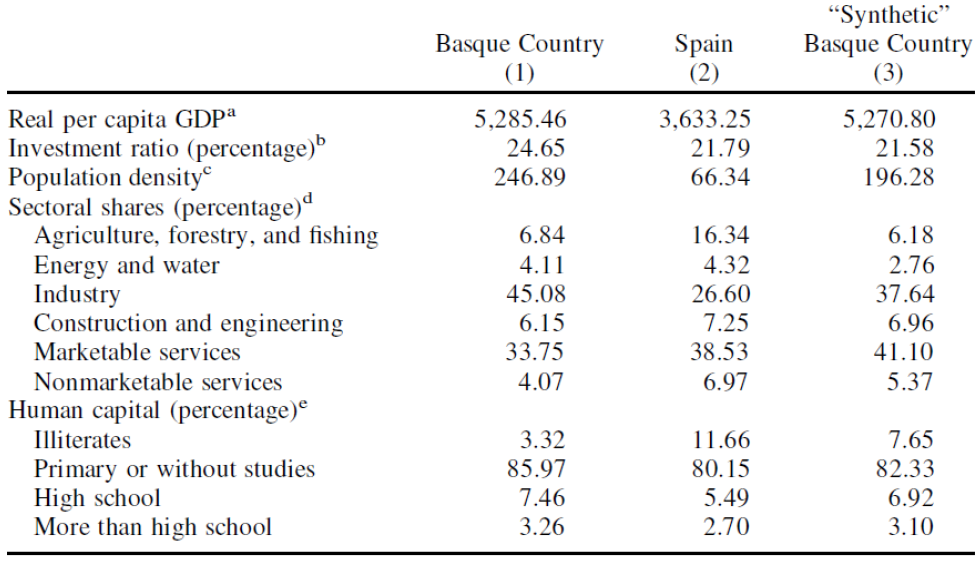
\includegraphics[width=0.8\linewidth]{./Figures/Basque}
\end{figure}

\end{frame}


\begin{frame}{Growth in the Basque with and without Terrorism}
\begin{figure}
\centering
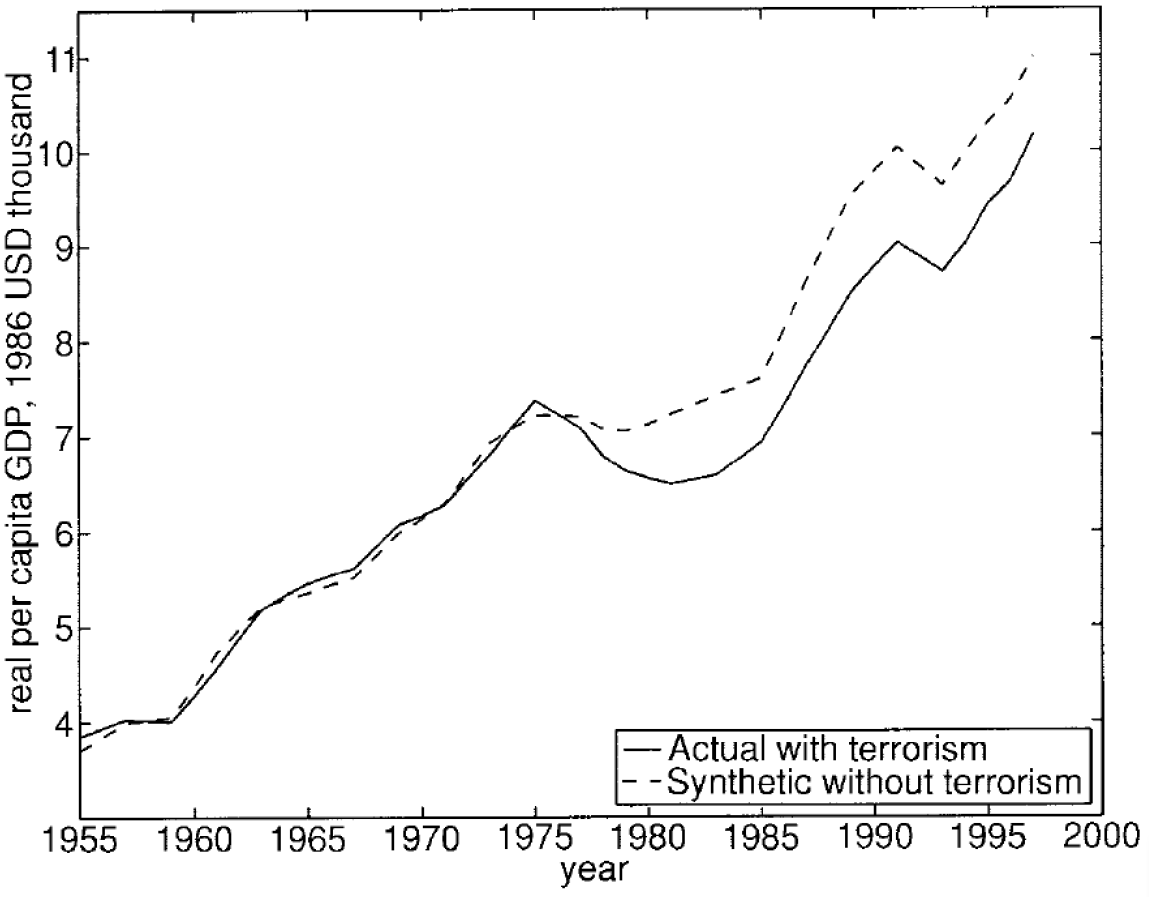
\includegraphics[width=0.8\linewidth]{./Figures/Basque2}
\caption{}
\label{fig:basque2}
\end{figure}
\end{frame}

%\subsection{Combining IV and DiD}
%\begin{frame}{Combining IV and DiD - Waldinger (2010)}
%	Question: The effect of faculty quality on the outcomes of PhD students.\medskip
%	
%	It is challenging because of:
%	\begin{enumerate}
%		\item Selection of good students into good universities.
%		\item Omitted variables affecting both faculty quality and student outcomes.
%		\item Measurement error in faculty quality.
%	\end{enumerate}\medskip
%
%	Waldinger (2010) uses the dismissal of scientists in Nazi Germany as an exogenous shock to faculty quality.
%	\begin{itemize}
%		\item Germany was the leading country for scientific research in early 1900.
%		\item In 1933 the new Nazi government dismissed all Jewish and `politically unreliable' scholars from the German universities.
%	\end{itemize}\medskip
%	
%	The dismissal affected some departments very strongly, while other departments were not affected.
%\end{frame}
%
%\begin{frame}{Dismissed Professors Across German Universities}
%	\begin{figure}
%		\centering
%		
\includegraphics[width=1\linewidth]{./Figures/waldinger1}
%	\end{figure}
%\end{frame}
%
%\begin{frame}{Effect of Dismissals on Faculty Size and Quality}
%	\begin{figure}
%		\centering
%		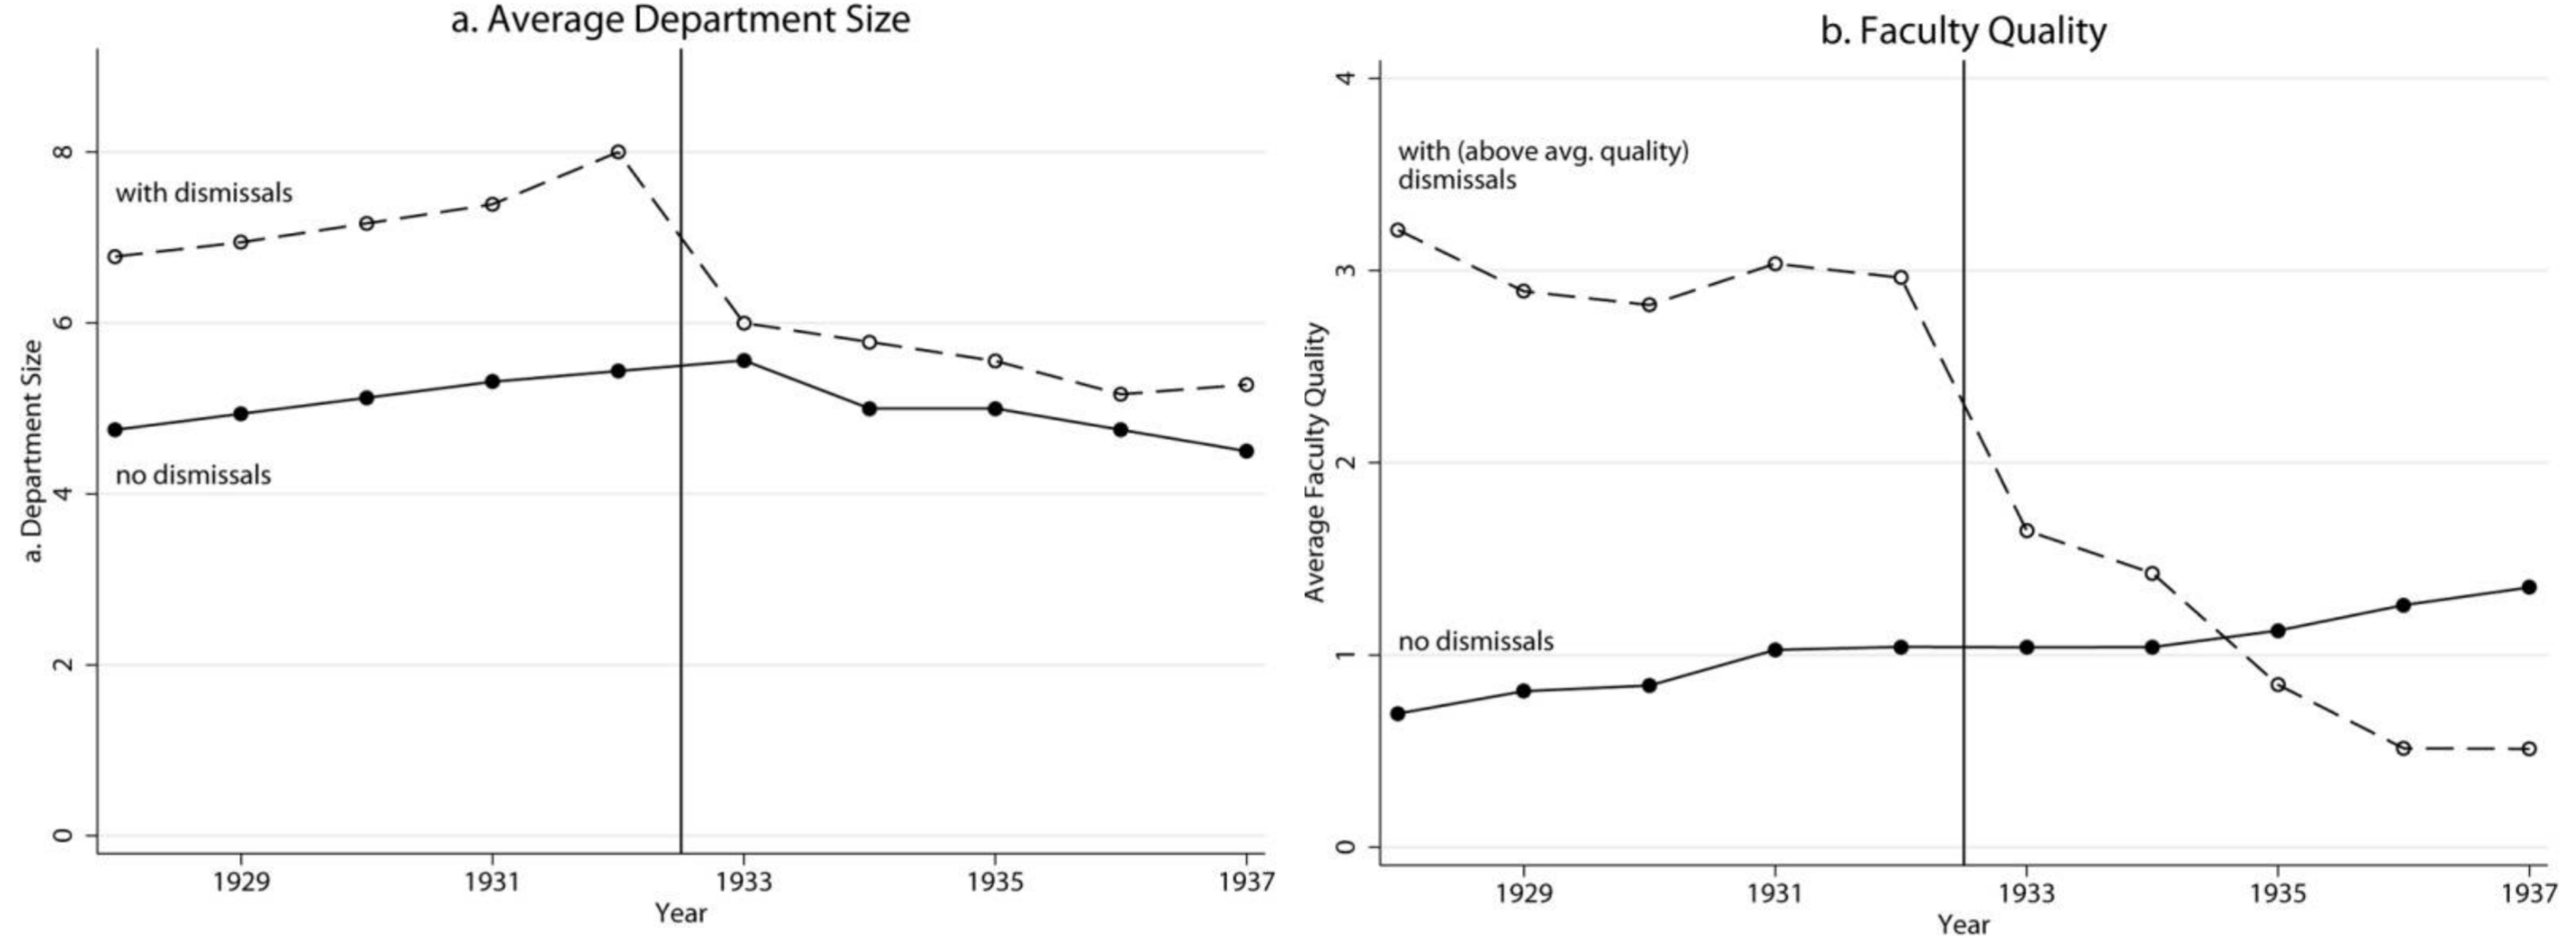
\includegraphics[width=1\linewidth]{./Figures/waldinger2}
%	\end{figure}
%	
%\end{frame}
%
%\begin{frame}{Reduced Form Graphical Analysis}
%	\begin{figure}
%		\centering
%		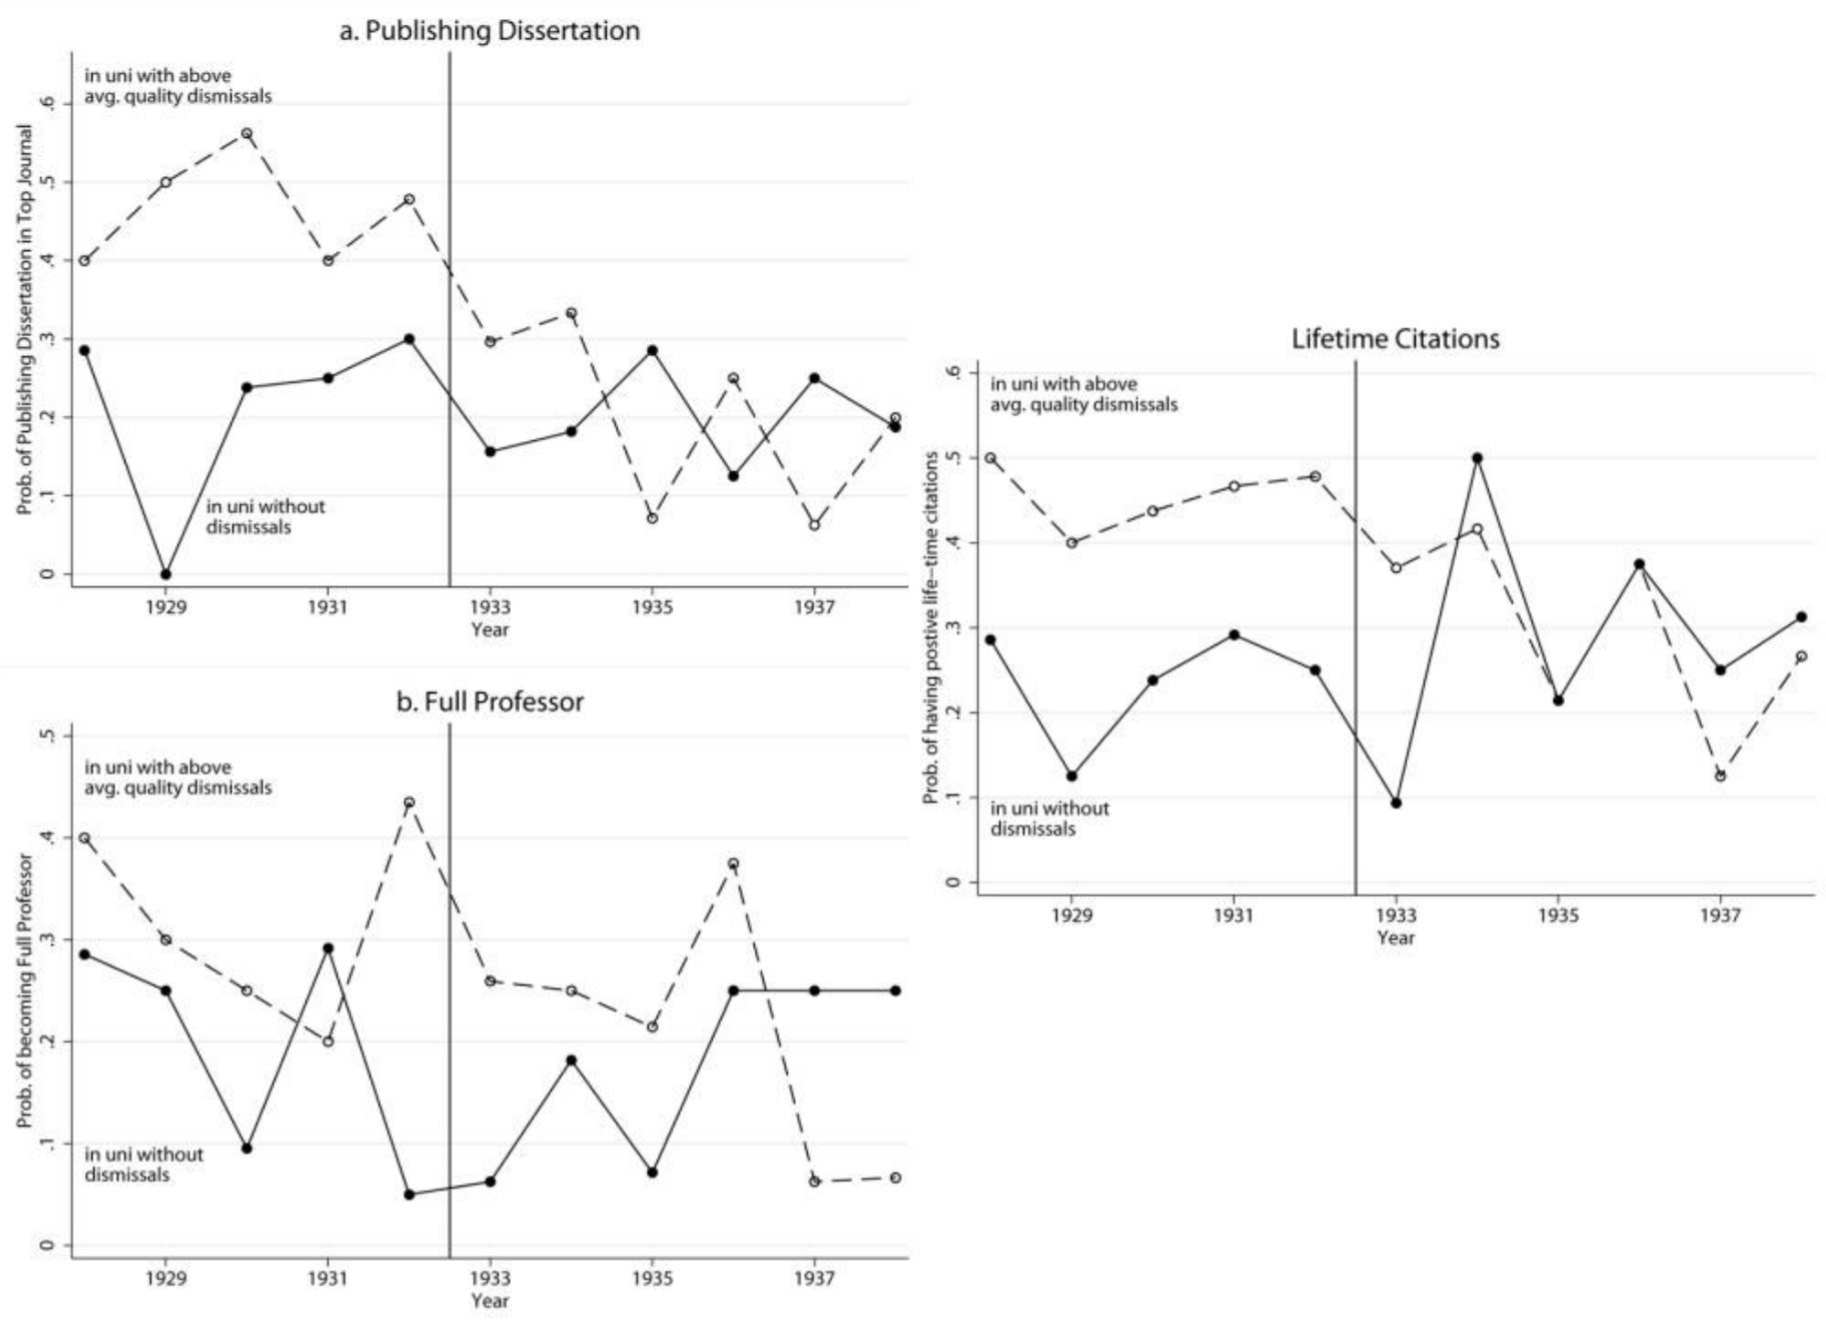
\includegraphics[width=.9\linewidth]{./Figures/waldinger3}
%	\end{figure}
%\end{frame}
%
%\begin{frame}{Reduced-form estimate}
%	\begin{figure}
%		\centering
%		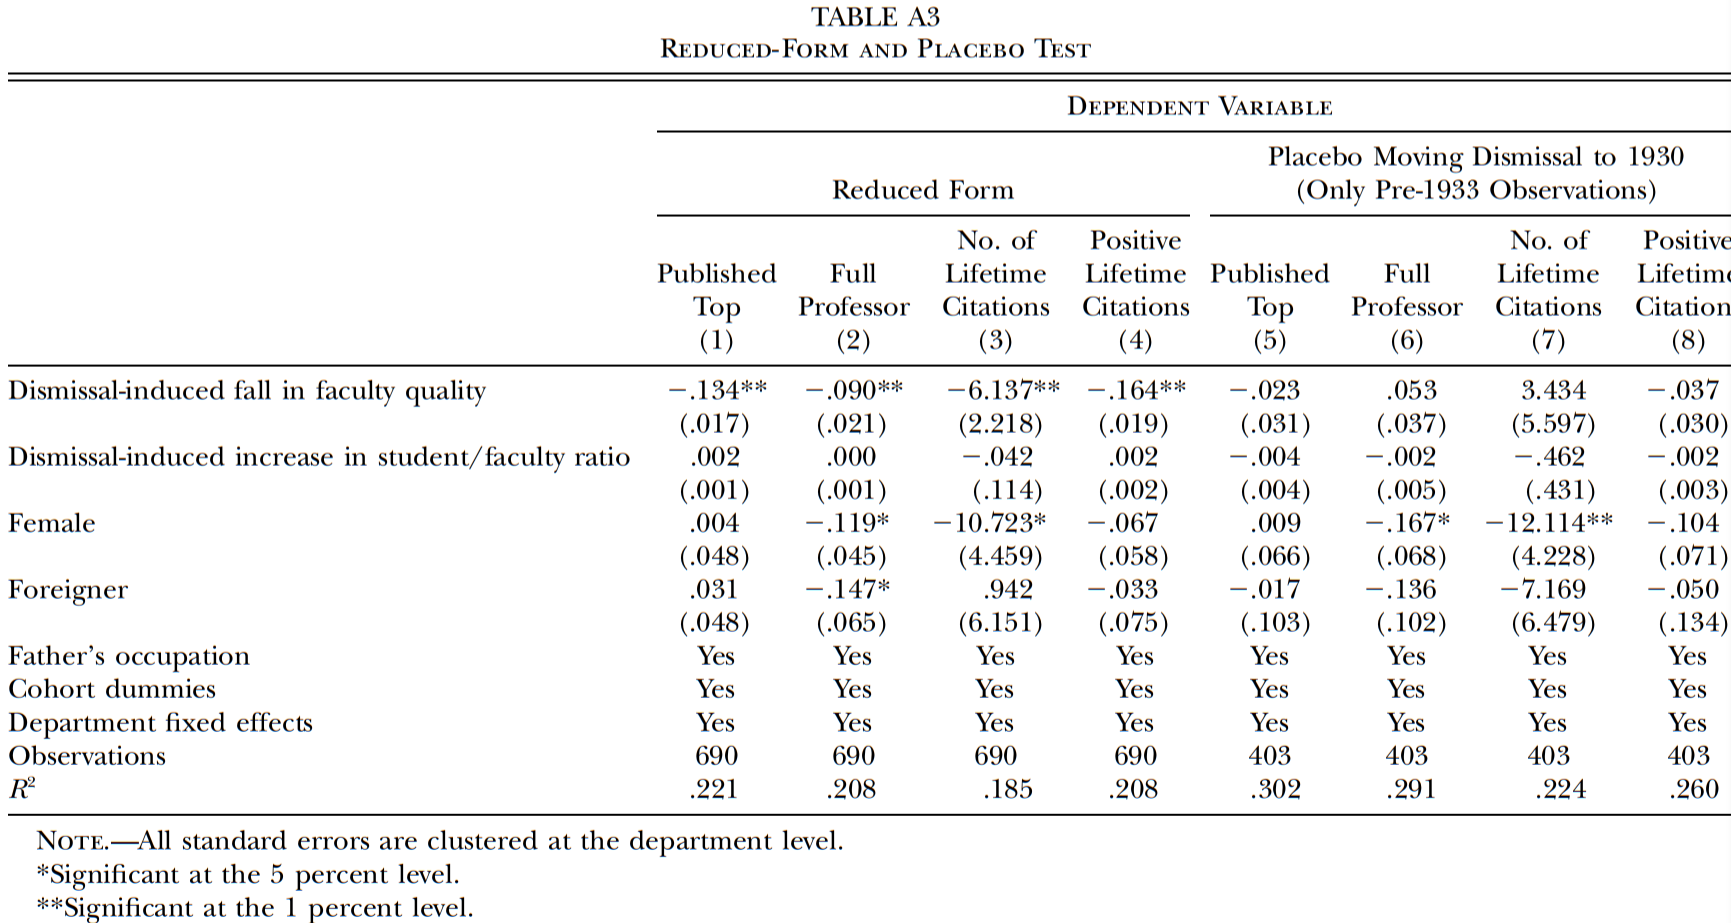
\includegraphics[width=.9\linewidth]{./Figures/waldinger4}
%	\end{figure}
%(5)-(8) are checks for Parallel Trend Assumption.	
%\end{frame}
%
%\begin{frame}{Using dismissal as IV}
%	The effect of university quality on PhD student outcomes:
%	
%	$\text{Outcome}_{idt} = b_1 + b_2(\text{Faculty Quality})_{dt-1}+b_3(\text{Student/Faculty Ratio})_{dt-1}$
%	
%	$\qquad \qquad + b_4 \text{Female}_{idt} + b_5 \text{Foreign}_{idt} + b_6 \text{CohortFE}_t + b_7 \text{DepFE}_d + \varepsilon_{idt}$
%	\medskip
%	
%	University quality and student/faculty ratio are endogenous $\rightarrow$ use dismissal as IV.\medskip
%	
%	First Stage Regressions:
%\begin{itemize}
%	\item $X_{idt} = g_1$
%		
%		+ $g_2(\text{Dismissal induced Reduction in Faculty Quality})_{dt}$
%		
%		+ $g_3(\text{Dismissal induced increase in Student/Faculty Ratio})_{dt}$
%		
%		+ $g_4 \text{Female}_{idt} + g_5 \text{Foreign}_{idt} + g_6 \text{CohortFE}_t + g_7 \text{DepFE}_d + \varepsilon_{idt}$
%		
%		\item Where $X_{idt}$ represents one of the two endogenous variables ``Faculty Quality'' and ``Student/Faculty Ratio''.
%\end{itemize} 
%
%\end{frame}
%
%
%\begin{frame}{First stage}
%	\begin{center}
%		
\includegraphics[width=0.7\linewidth]{./Figures/waldinger5}
%	\end{center}
%	To test for weak instruments because here we have 2 regressors and IVs use Cragg-Donald EV statistic here critical value is 7.03.
%\end{frame}
%
%\begin{frame}{Second stage}
%	\begin{figure}
%		\centering
%		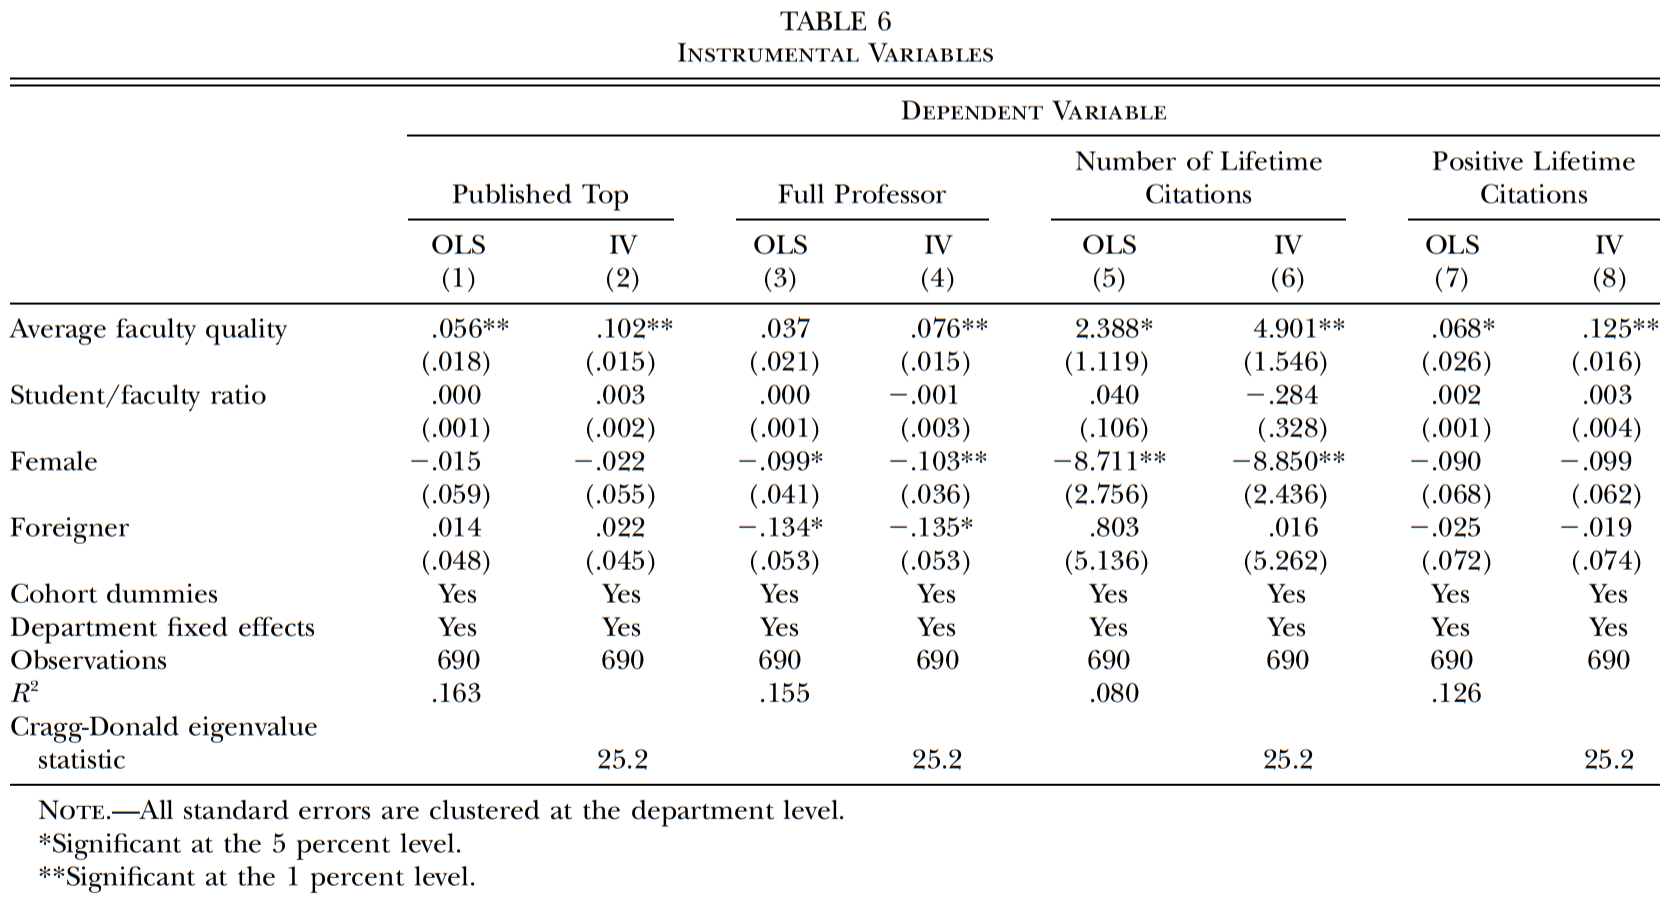
\includegraphics[width=1\linewidth]{./Figures/waldinger6}
%	\end{figure}
%\end{frame}
\section{References}
\tiny
\bibliographystyle{apalike}
\bibliography{./references}
\end{document}
